\section{Theoretical Analysis}
\label{sec:analysis}

In this section, the circuit shown in Figure \ref{fig:t2} is analysed
theoretically, analysing the circuit for $t<0$, calculating the equivalent resistance, determining the natural and forced solutions and superimposing them to find the total solution.

\subsection{Nodal analysis}
For t$<$0,  $v_s(t)= V_s(t)$,  it is a DC circuit. We can determine the voltges in all nodes and currents in all branches using the nodal method.
Since this is a linear circuit,  we apply Ohm's Law,  $V_i= R_i * I$ and the Kirchoff Current Law (KCL),  $\sum I_i = 0$.

We get the following equation,  in matrix form:

\begin{equation}
\label{eq:matrixeq1}
\begin{bmatrix}
    -G_1 & G_1+G_2+G_3 & -G_2 & 0 & -G_3 & 0 & 0 & 0\\
    0 & -G_2-K_b & G_2 & 0 & K_b & 0 & 0 & 0\\
    0 & K_b & 0 & 0 & -G_5-K_b & G_5 & 0 & 0\\
    0 & 0 & 0 & -G_6 & 0 & 0 & G_6+G_7 & -G_7\\
    1 & 0 & 0 & -1 & 0 & 0 & 0 & 0\\
    0 & 0 & 0 & 0 & 0 & 0 & 0 & 1\\
    0 & 0 & 0 & -K_c*G_6 & 1 & 0 & K_c*G_6 & -1\\
    0 & -G_3 & 0 & -G_4 & G_4+G_3+G_5 & -G_5 & -G_7 & G_7
\end{bmatrix}
\cdot
\begin{bmatrix}
V_1 \\
V_2 \\
V_3 \\
V_4 \\
V_5 \\
V_6 \\
V_7 \\
V_8 
\end{bmatrix}
=
\begin{bmatrix}
0 \\
0 \\
0 \\
0\\
V_s\\
0 \\
0 \\
0
\end{bmatrix}
\end{equation}


This equation solved using octave yields the following results:

\begin{table}[H]
    \centering
    \begin{tabular}{|l|r|}
      \hline    
      {\bf Variable} & {\bf Value [A or V]} \\ \hline
      $V_1$ & $5.13612248730V$ \\ \hline 
$V_2$ & $4.88464690881V$ \\ \hline 
$V_3$ & $4.36195145882V$ \\ \hline 
$V_4$ & $-0.00000000000V$ \\ \hline 
$V_5$ & $4.92000960269V$ \\ \hline 
$V_6$ & $5.69027079572V$ \\ \hline 
$V_7$ & $-1.96654083449V$ \\ \hline 
$V_8$ & $-2.94453891610V$ \\ \hline 
$I_1$ & $0.00024147744A$ \\ \hline 
$I_2$ & $0.00025321233A$ \\ \hline 
$I_3$ & $-0.00001173489A$ \\ \hline 
$I_4$ & $-0.00120106056A$ \\ \hline 
$I_5$ & $-0.00025321233A$ \\ \hline 
$I_6$ & $0.00095958312A$ \\ \hline 
$I_7$ & $0.00095958312A$ \\ \hline 
$I_S$ & $-0.00024147744A$ \\ \hline 
$I_b$ & $-0.00025321233A$ \\ \hline 
$I_c$ & $-0.00000000000A$ \\ \hline 
$I_e$ & $-0.00095958312A$ \\ \hline
    \end{tabular}
    \caption{Node Analysis Results for t$<$0}
    \label{tab:nodeanalysis}
  \end{table}
  
  
\subsection{Equivalent resistance}
Now,  we have to determine the equivalent resistance $R_{eq}$ as seen from the capacitor terminals. We take out all the independent voltage sources (make $v_s=0$) and replace the capacitor with a voltage source $Vx= V(6)-V(8)$. The values of$ V(6)$ and $V(8)$ were already obtained via nodal analysis in the previous subsection. To determine the current $I_x$ supplied by $V_x$ we run mesh analysis. This is necessary because the resistors are arranged in such a way that they cannot be simplified into an equivalent resistor by applying the usual equations for resistors in series and in parallel. The mesh method gives us these equations in matriz form:


\begin{equation}\label{eq:matrixeq2}
\begin{bmatrix}
 R_1+R_3+R_4 & -R_3 & -R_4 & 0\\
    -K_bR_3 &  K_bR_3-1 & 0 & 0\\ 
    -R_4 & 0 & R_4+R_6+R_7-K_d & 0\\
    0 & -R_5 & K_d & R_5 
\end{bmatrix}
\cdot
\begin{bmatrix}
I_A\\
I_B \\
I_C \\
I_D \\

    \end{bmatrix}
=
    \begin{bmatrix}
0 \\
0 \\
0 \\
V_x \\

    \end{bmatrix}
  \end{equation}

This yields the following results:

\begin{table}[H]
    \centering
    \begin{tabular}{|l|r|}
      \hline    
      {\bf Variable} & {\bf Value [A or V]} \\ \hline
      V_x & 8.63480971182V \\ \hline 
I_x & 0.00283856995V \\ \hline 
R_{equiv} & 3041.95770117000V \\ \hline 

    \end{tabular}
    \caption{Equivalent resistance}
    \label{tab:equivalentresistance}
  \end{table}


For the time constant:

$\tau = R_{eq} \cdot C = 0.00313933181s$







\subsection{Natural solution}

Using the capacitor voltage $V_x$ for $t<0$ as the initial condition, the natural solution of $v_{6n}(t)$ becomes:

\begin{equation}
\label{eq:solucaonatural}
v_{6n}(t)=V_x e^{\frac{-t}{R_{eq}C}}
\end{equation}

This equation gives us the following plot in [0,20]ms:

  \begin{figure}[H] \centering
    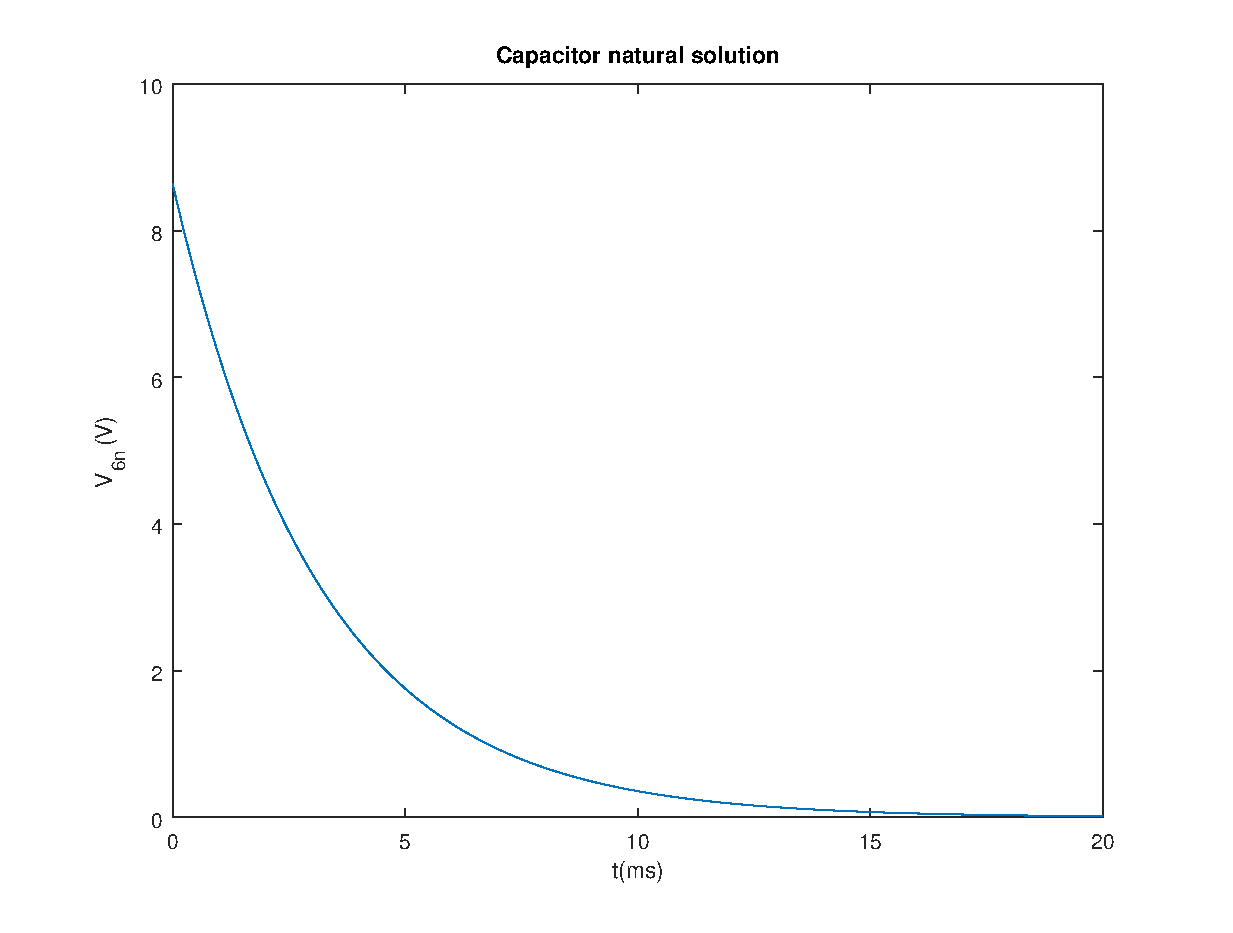
\includegraphics[width=1\linewidth]{natural.eps}
    \caption{Natural solution $v_{6n}(t)$}
    \label{fig:natural}
    \end{figure}



\subsection{Forced solution}

To determine the forced solution in the same interval [0, 20]ms we use a phasor voltage source $V_s$ and replace $C$ with its impedance $Z_c$.

We run nodal analysis to determine the phasor voltages in all nodes:

 $\omega=2\pi f$
 
\small
  \begin{equation}\label{eq:matrixeq3}
\begin{bmatrix}
-G_1 & G_1+G_2+G_3 & -G_2 & 0 & -G_3 & 0 & 0 & 0\\
0 & -G_2-K_b & G_2 & 0 & K_b & 0 & 0 & 0\\
0 & K_b & 0 & 0 & -G_5-K_b & G_5+(j\omega C) & 0 & -(j\omega C)\\
0 & 0 & 0 & -G_6 & 0 & 0 & G_6+G_7 & -G_7\\
1 & 0 & 0 & -1 & 0 & 0 & 0 & 0\\
0 & 0 & 0 & 1 & 0 & 0 & 0 & 0\\
0 & 0 & 0 & -K_dG_6 & 1 & 0 & K_dG_6 & -1\\
0 & -G_3 & 0 & -G_4 & G_4+G_3+G_5 & -G_5-(j\omega C) & -G_7 & G_7+(j \omega C)
\end{bmatrix}
\cdot
\begin{bmatrix}
V_{1p} \\
V_{2p} \\
V_{3p} \\
V_{4p} \\
V_{5p} \\
V_{6p} \\
V_{7p} \\
V_{8p} 
    \end{bmatrix}
=
    \begin{bmatrix}
0 \\
0 \\
0 \\
0 \\
i \\
0 \\
0 \\
0 
    \end{bmatrix}
  \end{equation}

\small
Solving this system of equation in octave yields the following results:

\begin{table}[H]
    \centering
    \begin{tabular}{|l|r|}
      \hline    
      {\bf Variable} & {\bf Value [A or V]} \\ \hline
      $\tilde{V}_1$ & $(0.00000000000+i\cdot1.00000000000)V$ \\ \hline 
$\tilde{V}_2$ & $(0.00000000000+i\cdot0.95103785412)V$ \\ \hline 
$\tilde{V}_3$ & $(0.00000000000+i\cdot0.84926936022)V$ \\ \hline 
$\tilde{V}_4$ & $(0.00000000000+i\cdot0.00000000000)V$ \\ \hline 
$\tilde{V}_5$ & $(0.00000000000+i\cdot0.95792294963)V$ \\ \hline 
$\tilde{V}_6$ & $(0.08501303490+i\cdot-0.56899006711)V$ \\ \hline 
$\tilde{V}_7$ & $(-0.00000000000+i\cdot-0.38288433334)V$ \\ \hline 
$\tilde{V}_8$ & $(-0.00000000000+i\cdot-0.57329997939)V$ \\ \hline
    \end{tabular}
    \caption{Phasor voltages}
    \label{tab:phasorvoltages}
  \end{table}
  
  

\subsection{Total solution}

Converting the phasors to real time functions for f=1KHz, we can then superimpose the natural and forced solutions:

$v_6(t)=V_xe^{\frac{-t}{R_{eq}C}}-\Re(\tilde{V_6}e^{j\omega t})$


  This plot in the interval [-5,20]ms:

  \begin{figure}[H] \centering
    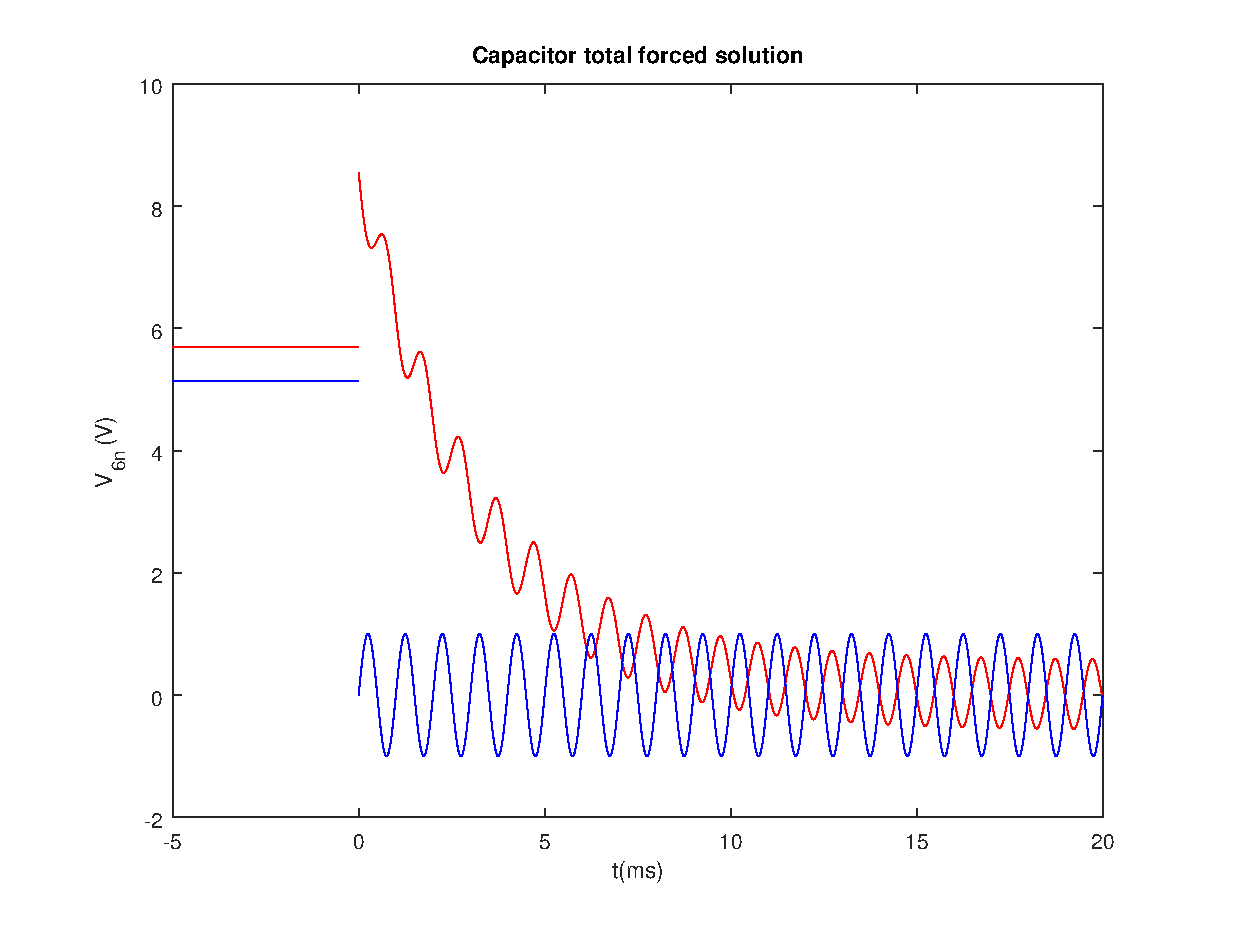
\includegraphics[width=1\linewidth]{forced.eps}
    \caption{Final total solution $v_{6}(t)$}
    \label{fig:total}
    \end{figure}
    
\subsection{Frequency responses}
      
The system \ref{eq:matrixeq3} was solved for various values of $f$.
The plots of the magnitude and phase of $V_s$, $V(6)$ and $V_C$, for
values ranging from $0.1 Hz$ to $1 MHz$ are below:

    \begin{figure}[H] \centering
    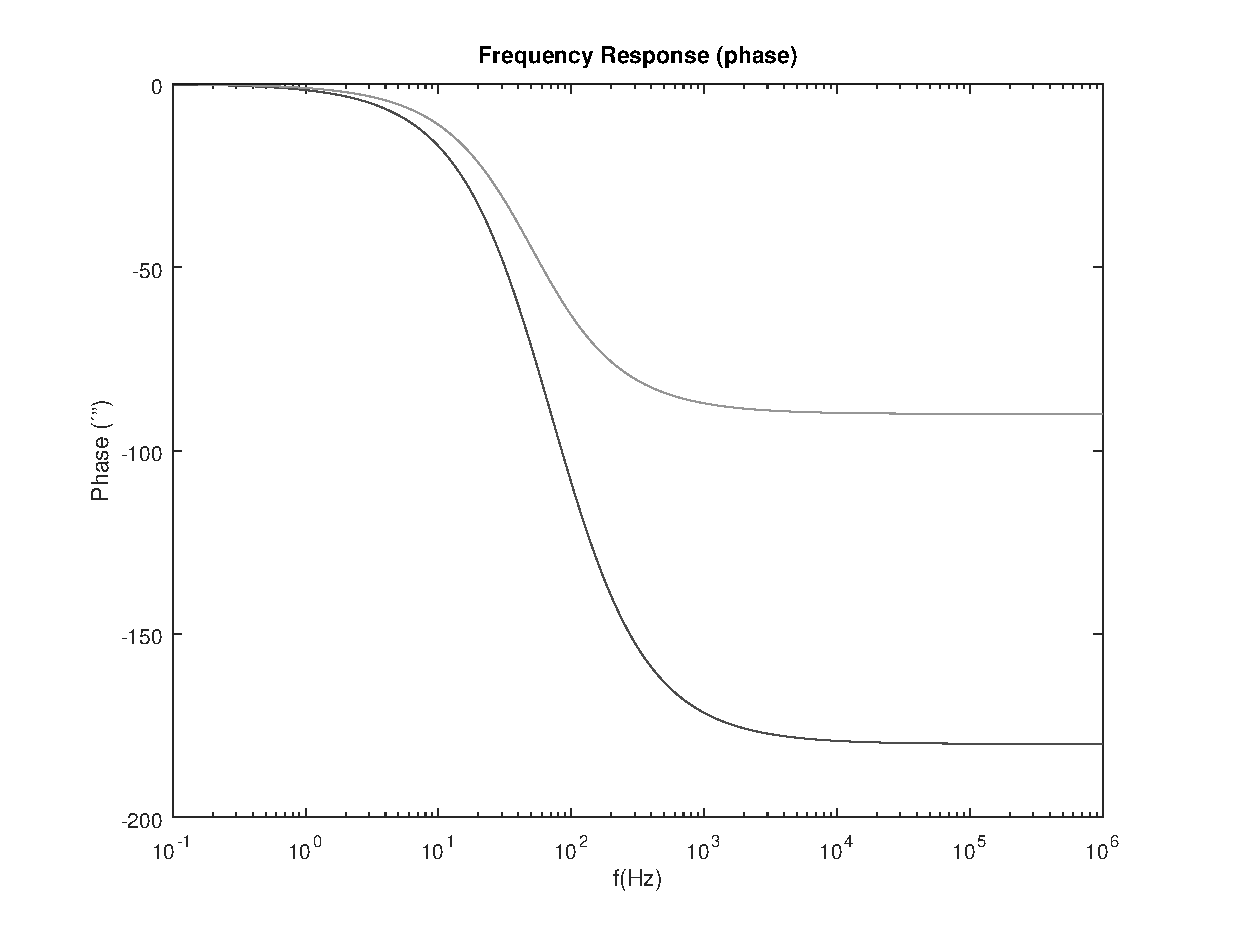
\includegraphics[width=1\linewidth]{degree.eps}
    \caption{Frequency response-phase}
    \label{fig:frequencyresponsephase}
    \end{figure}
    
      \begin{figure}[H] \centering
    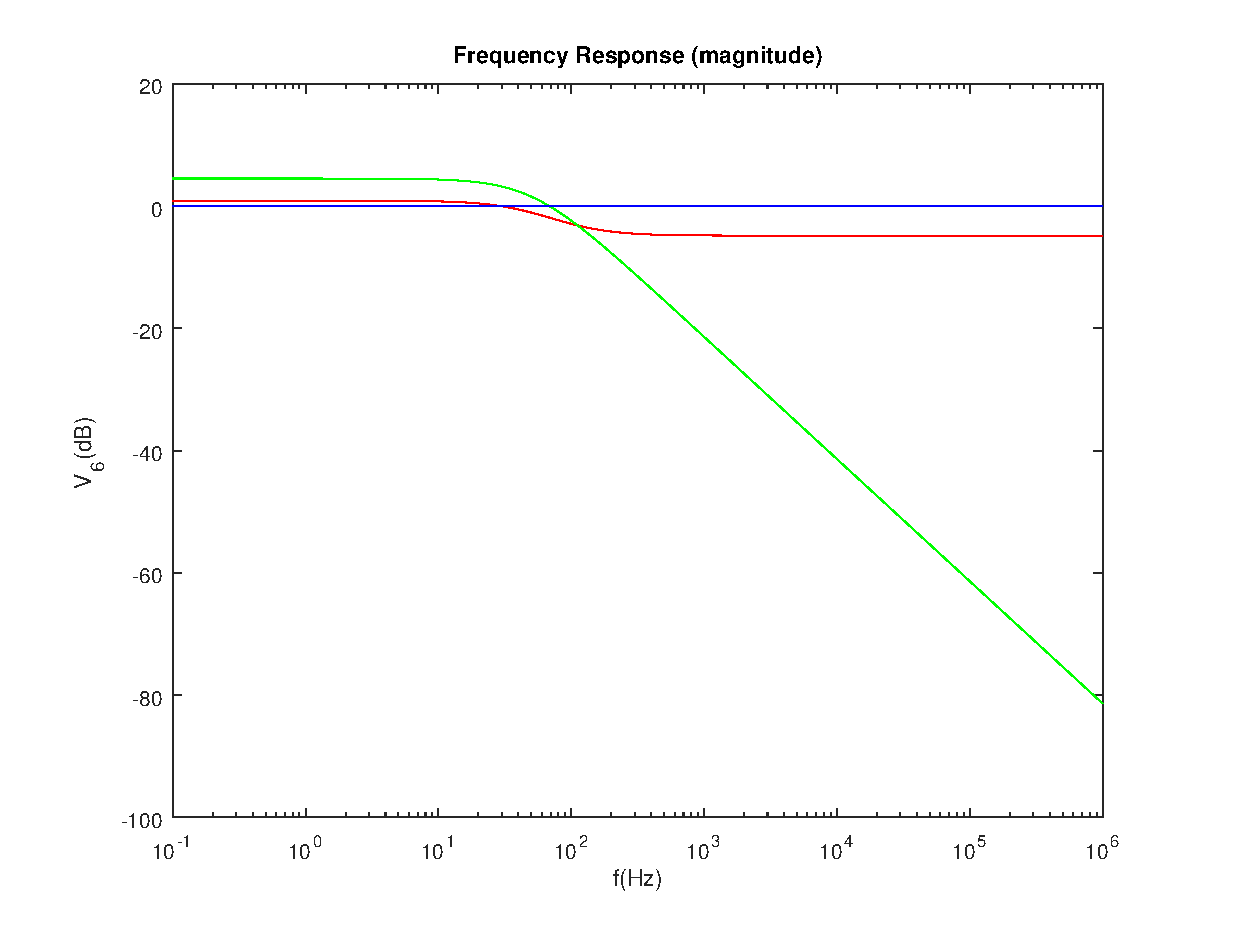
\includegraphics[width=1\linewidth]{dB.eps}
    \caption{Frequency response-magnitude}
    \label{fig:frequencyresponsemagnitude}
    \end{figure}
  